\documentclass[preprint,12pt]{elsarticle}

\usepackage{amsmath,amssymb}
\usepackage{graphicx}
\usepackage{booktabs}
\usepackage{hyperref}
\usepackage{url}
\usepackage{tikz}
\usetikzlibrary{arrows.meta,positioning}

\graphicspath{{../figures/}}

\journal{Computer Physics Communications}

\begin{document}

\begin{frontmatter}

\title{PIC Deposition Benchmark Suite: A Reproducible Reference for Charge Deposition in Two-Dimensional Electrostatic Particle-In-Cell Simulations}

\author[inst]{Elhadj Hocine}
\ead{hocineelhadj@gmail.com}
\address[inst]{Independent Researcher}

\begin{abstract}
Charge deposition dominates cost and accuracy in explicit Particle-In-Cell (PIC) plasma simulations.
We present an open-source 2D electrostatic reference program that evaluates Nearest Grid Point (NGP), Cloud-In-Cell (CIC), Triangular-Shaped Cloud (TSC), and Esirkepov deposition under cache-aware CPU optimizations and optional CUDA backends.
The suite separates cell-sort cost from deposit-kernel throughput, profiles full PIC timesteps (push, sort, deposit, Poisson solve, gather), and bundles charge, energy, spectral-noise, Langmuir-wave, two-stream, and long-run conservation validation.
Benchmarks on Apple M1 Pro and Tesla T4 (same-host CPU baseline) show deposition is memory-bandwidth limited; CIC offers the best CPU accuracy--performance trade-off and GPU atomics are preferred at large particle counts on T4.
Archived CSV pipelines regenerate all figures.
Source code and data are available at \url{https://github.com/ehocine/pic-deposition} (Zenodo DOI: \texttt{TODO-DOI}).
\end{abstract}

\begin{keyword}
Particle-In-Cell \sep charge deposition \sep benchmark \sep reproducibility \sep GPU \sep plasma simulation
\end{keyword}

\end{frontmatter}

\section*{Program Summary}

\noindent\textbf{Program Title:} PIC Deposition Benchmark Suite (2D electrostatic reference)\\
\textbf{Developer's repository link:} \url{https://github.com/ehocine/pic-deposition}\\
\textbf{Licensing provisions:} MIT license\\
\textbf{Programming language:} C++17; optional CUDA\\
\textbf{Supplementary material:} Archived benchmark CSVs in \texttt{data/benchmarks/}; figure scripts in \texttt{scripts/plot\_results.py}\\
\textbf{Journal Reference of previous version:} Not applicable\\
\textbf{Does the new version supersede the previous version?:} Not applicable

\subsection*{Nature of problem}
Explicit Particle-In-Cell (PIC) simulations spend a large fraction of each timestep in charge deposition: irregular, scatter-oriented updates from macroparticles to a structured grid.
Practitioners must choose among deposition schemes (NGP, CIC, TSC, Esirkepov) and implementation strategies (particle layout, sorting, CPU privatization, GPU atomics) while preserving charge conservation and controlling grid noise over thousands of timesteps.
A reproducible reference that isolates deposition-kernel performance and couples it to standard physics diagnostics is needed to compare schemes before porting kernels into production PIC codes such as PIConGPU or Smilei.

\subsection*{Solution method}
The program implements a 2D electrostatic PIC cycle with FFT-based Poisson solve, four deposition schemes behind a unified \texttt{DepositionConfig} interface, and separate timing of cell sorting versus deposit-kernel execution.
OpenMP thread-local grid privatization is provided for CPU runs; CUDA backends implement global atomics and multi-block spatial-tile privatization for CIC.
Bundled executables (\texttt{pic\_test}, \texttt{pic\_benchmark}, \texttt{pic\_validation}, \texttt{pic\_sim}) run microbenchmarks, full-timestep profiles, Langmuir-wave and two-stream validation, and long-run conservation studies.
Results are written as CSV files and converted to publication figures via \texttt{scripts/plot\_results.py}.

\subsection*{Additional comments including Restrictions and Unusual features}
The code targets 2D electrostatic problems on a unit-square periodic domain; electromagnetic current deposition, MPI domain decomposition, and 3D stencils are not included.
GPU benchmarks require CUDA (\texttt{BUILD\_CUDA=ON}) or the provided Kaggle script; cross-platform CPU (Apple M1 Pro) and GPU (Tesla T4) results must be interpreted with explicit hardware labels.
Esirkepov deposition uses deposit$\rightarrow$solve$\rightarrow$push$\rightarrow$gather (trajectory deposit at step start, position advance with pre-field velocity, then velocity update).
The multi-block GPU privatized kernel preserves charge conservation but scans all particles per spatial tile and is slower than atomics on tested grids.
A Zenodo DOI (\texttt{TODO-DOI}) will be assigned at release.


\section{Introduction}
\label{sec:intro}

Particle-In-Cell (PIC) methods combine Lagrangian macroparticles with Eulerian field grids and are central to kinetic plasma simulation~\cite{birdsall1991,hockney1988,dawson1983}.
Each explicit timestep performs particle push, charge deposition, field solve, and field gather; deposition is frequently the performance bottleneck because it performs irregular scatter writes to a structured grid~\cite{viereck2016}.
Long-time accuracy additionally requires that deposited charge preserve global conservation to machine precision or via trajectory-based schemes~\cite{brackbill1980,esirkepov2001}; poor conservation injects spurious fields and energy drift over thousands of timesteps.

Production codes such as PIConGPU~\cite{burau2010,steiniger2023} and Smilei~\cite{derouillat2018,beck2019} integrate deposition into large-scale 3D electromagnetic workflows with MPI, I/O, and architecture-specific GPU kernels.
Practitioners nonetheless need a compact, reproducible reference to compare NGP, CIC, TSC, and Esirkepov under controlled 2D electrostatic settings with explicit sort-versus-deposit timing and bundled validation diagnostics before adapting kernels to production environments.

This program provides:
\begin{itemize}
    \item A unified C++17 deposition interface with AoS/SoA layouts, optional cell sorting, OpenMP privatization, and CUDA atomics or tiled privatization.
    \item Microbenchmarks, full-timestep profiles, roofline-style analysis, and archived CSV regeneration of all figures.
    \item Physics validation: Langmuir-wave frequency agreement, two-stream growth-rate agreement, and 2000-step conservation studies.
\end{itemize}

Section~\ref{sec:related} reviews related PIC deposition work.
Section~\ref{sec:methods} summarizes schemes (inherited notation from the methods section).
Sections~\ref{sec:program}--\ref{sec:install} document program structure and installation.
Sections~\ref{sec:methodology}--\ref{sec:results} present benchmarks; Section~\ref{sec:physics} reports validation; Section~\ref{sec:code_comparison} compares with literature.

\section{Related Work}
\label{sec:related}

\subsection{Classical deposition and conservation}
Early PIC studies established that grid resolution and shape-function choice control aliasing noise and numerical heating~\cite{langdon1970,okuda1972}.
Brackbill and Barnes showed that discrete charge non-conservation can destabilize long-time integrations~\cite{brackbill1980}, motivating exact deposition schemes.
Esirkepov's trajectory-based method provides rigorous charge conservation for arbitrary shape factors~\cite{esirkepov2001}, while Eastwood's virtual-particle formulation extended conservative deposition to electromagnetic PIC~\cite{eastwood1981}.

\subsection{Production PIC codes}
PIConGPU~\cite{burau2010,huebl2019} targets large-scale electromagnetic PIC on heterogeneous supercomputers, combining Esirkepov or EZ (Esirkepov-meets-ZigZag) current deposition~\cite{steiniger2023} with supercell-local caching strategies that reduce global atomic contention on GPUs.
Smilei~\cite{derouillat2018} couples cycle-sort particle reordering with SIMD-vectorized deposition and gathering; Beck et al.\ report operator speedups of up to $\sim$3$\times$ when sorting enables vectorized projection at sufficient particles-per-cell~\cite{beck2019}.
Both codes address production-scale 3D electromagnetic physics; they do not provide a compact, deposition-focused reference for comparing NGP/CIC/TSC/Esirkepov under identical 2D electrostatic settings with separated sort and deposit timing.

\subsection{Hybrid and GPU deposition engineering}
Harvey et al.\ implemented charge-conserving deposition on hybrid CPU--GPU systems and reported up to $\sim$4$\times$ GPU speedup over a CPU baseline for tiled privatized deposition on tested hybrid nodes~\cite{harvey2015}.
Viereck et al., in a CPC survey of emerging architectures, concluded that PIC scatter operations are memory-bandwidth limited and that privatized or tiled accumulation can outperform naive atomics when contention is high, but that the optimal strategy is architecture dependent~\cite{viereck2016}.
Wilke et al.\ discussed GPU PIC strategies for exascale systems~\cite{wilke2017}; Huebl et al.\ analyzed CPU/GPU cluster scalability of the PIConGPU deposition pipeline~\cite{huebl2014}.
Our roofline-style analysis and separate M1 versus T4-host reporting follow Viereck's recommendation to treat deposition as a memory problem rather than a floating-point ceiling problem.

\subsection{This program's niche}
The present program is a lightweight 2D electrostatic reference for deposition research and teaching: four schemes behind one runtime interface, explicit separation of sort and deposit-kernel timing, bundled charge/energy/spectral/Langmuir/two-stream/conservation diagnostics, and archived CSV pipelines for figure regeneration.
It is not a replacement for PIConGPU or Smilei in production laser-plasma or exascale campaigns; it is intended as a reproducible benchmark suite for scheme, layout, sorting, and backend selection prior to porting kernels into larger codes.

\section{Deposition Methods}
\label{sec:methods}
Charge deposition maps $N_p$ macroparticles onto an $N_x \times N_y$ grid by scattering weighted contributions into $\rho$.
Each scheme trades stencil width, arithmetic cost, and spectral smoothness.
Table~\ref{tab:stencil} summarizes the per-particle grid touches in our 2D implementation.

\begin{table}[t]
\centering
\caption{Deposition stencil characteristics in 2D.}
\label{tab:stencil}
\begin{tabular}{lrrl}
\toprule
Scheme & Nodes & Writes/particle & Conservation \\
\midrule
NGP  & 1  & 1 & Point assignment \\
CIC  & 4  & 4 & Not exact; low error \\
TSC  & 9  & 9 & Not exact; lowest noise \\
Esirkepov & $\mathcal{O}(L)$ & $\mathcal{O}(L^2)$ & Exact along trajectory \\
\bottomrule
\end{tabular}
\end{table}
\noindent$L$ is the number of grid cells crossed by the particle trajectory in one dimension.

\subsection{Nearest Grid Point (NGP)}
NGP assigns each macroparticle charge $q_p$ to the nearest grid node $(j_x,j_y)$.
Given fractional cell coordinates $(w_x,w_y)$ from the particle position,
\begin{equation}
    j_x = \begin{cases} i_x+1 & w_x \geq 0.5 \\ i_x & \text{otherwise} \end{cases},
\end{equation}
with analogous rule for $j_y$, and update
\begin{equation}
    \rho_{j_x,j_y} \mathrel{+}= \frac{q_p}{\Delta x\,\Delta y}.
\end{equation}
NGP performs one read-modify-write per particle and is the fastest scheme, but its discontinuous shape function injects the highest grid noise.

\subsection{Cloud-In-Cell (CIC)}
CIC distributes charge to the four nodes of the host cell using separable linear weights.
For one dimension,
\begin{equation}
    w_1 = 1-\xi, \qquad w_2 = \xi, \qquad \xi = \frac{x_p-x_i}{\Delta x},
\end{equation}
and in 2D,
\begin{equation}
    \rho_{i,j} \mathrel{+}= \frac{q_p}{\Delta x\,\Delta y}
    \sum_{\alpha,\beta \in \{0,1\}} w_x^{(\alpha)} w_y^{(\beta)},
\end{equation}
where $w_x^{(0)}=1-w_x$, $w_x^{(1)}=w_x$, and similarly for $y$.
CIC is the standard production choice: four grid writes per particle with substantially lower high-$k$ noise than NGP.

\subsection{Triangular-Shaped Cloud (TSC)}
TSC uses a three-point quadratic B-spline per dimension, touching nine nodes in 2D.
With normalized coordinate $\xi = x_p/\Delta x$ and base index $i_0 = \lfloor \xi - 0.5 \rfloor$,
let $x = \xi - i_0$. The weights are
\begin{align}
    w_0(x) &= \tfrac{1}{2}(1.5-x)^2, \\
    w_1(x) &= 0.75 - (x-1)^2, \\
    w_2(x) &= \tfrac{1}{2}(x-0.5)^2.
\end{align}
The 2D deposit is the tensor product $w_x^{(d_x)} w_y^{(d_y)}$ over $d_x,d_y \in \{0,1,2\}$.
TSC reduces spectral noise relative to CIC at the cost of nine scatter writes and additional weight arithmetic.

\subsection{Esirkepov Charge-Conserving Deposition}
Esirkepov's scheme deposits charge along the particle trajectory so that the discrete charge density update is exactly conservative~\cite{esirkepov2001}.
For a particle moving from $\mathbf{x}_0$ to $\mathbf{x}_1 = \mathbf{x}_0 + \mathbf{v}\,\Delta t$ over one timestep,
1D trajectory weights $W_i$ are accumulated by marching through crossed cell boundaries:
\begin{equation}
    W_i \mathrel{+}= \frac{x_{\mathrm{next}} - x_{\mathrm{curr}}}{\Delta x},
\end{equation}
where $x_{\mathrm{next}}$ is clipped to the next cell face or the endpoint.
In 2D we form separable weights $W^x_i$ and $W^y_j$ and deposit only over the sparse outer product of nonzero supports:
\begin{equation}
    \rho_{i,j} \mathrel{+}= \frac{q_p}{\Delta x\,\Delta y}\, W^x_i\, W^y_j.
\end{equation}
Our implementation stores only cells touched by the trajectory, giving $\mathcal{O}(L_x L_y)$ writes per particle where $L_x$ and $L_y$ are the number of cells crossed in each dimension.

\section{Program structure}
\label{sec:program}

\subsection{Executables}
Four command-line executables are built from a static library \texttt{pic\_core}:
\begin{itemize}
    \item \texttt{pic\_sim}: interactive full-PIC runs.
    \item \texttt{pic\_benchmark}: parameter-matrix sweeps and CSV output (\texttt{--timestep}, \texttt{--validate}, \texttt{--conservation}, \texttt{--gpu}).
    \item \texttt{pic\_validation}: Langmuir, conservation, and two-stream diagnostics.
    \item \texttt{pic\_test}: unit tests for charge conservation (CPU and optional CUDA).
\end{itemize}

\subsection{Module architecture}
Figure~\ref{fig:architecture} shows data flow.
\texttt{ParticlesSoA}/\texttt{ParticlesAoS} store macroparticle state; \texttt{FieldGrid} holds $\rho$, $\phi$, and $\mathbf{E}$.
\texttt{DepositionConfig} selects scheme, layout, sorting, thread count, and backend at runtime.
\texttt{cell\_sort} reorders particles by cell index; deposition kernels in \texttt{src/deposition/} implement NGP, CIC, TSC, and Esirkepov for CPU and CUDA.
\texttt{PoissonSolverFFT} (FFTW) solves for $\phi$; gather and push routines complete the leapfrog cycle.

\begin{figure}[t]
\centering
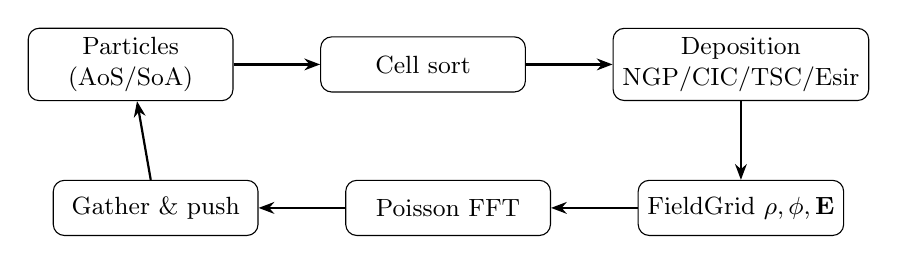
\begin{tikzpicture}[
    node distance=1.1cm,
    box/.style={draw, rounded corners, minimum width=2.6cm, minimum height=0.7cm, align=center, font=\small},
    arr/.style={-{Stealth[length=2mm]}, thick}
]
\node[box] (particles) {Particles\\(AoS/SoA)};
\node[box, right=of particles] (sort) {Cell sort};
\node[box, right=of sort] (deposit) {Deposition\\NGP/CIC/TSC/Esir};
\node[box, below=1.0cm of deposit] (grid) {FieldGrid $\rho,\phi,\mathbf{E}$};
\node[box, left=of grid] (poisson) {Poisson FFT};
\node[box, left=of poisson] (gather) {Gather \& push};
\draw[arr] (particles) -- (sort);
\draw[arr] (sort) -- (deposit);
\draw[arr] (deposit) -- (grid);
\draw[arr] (grid) -- (poisson);
\draw[arr] (poisson) -- (gather);
\draw[arr] (gather) -- (particles);
\end{tikzpicture}
\caption{Program data flow for one explicit PIC timestep (Esirkepov: deposit$\rightarrow$solve$\rightarrow$push$\rightarrow$gather).}
\label{fig:architecture}
\end{figure}

\subsection{Timestep cycle}
For NGP, CIC, and TSC the code pushes particles, optionally sorts, deposits charge, adds a neutralizing background when required by validation modes, solves Poisson's equation, and gathers fields to update velocities.
Esirkepov deposits along the particle trajectory using the pre-push position and displacement $\mathbf{v}_p\Delta t$, solves Poisson's equation, advances positions with the pre-field velocity, then gathers fields to update velocities for the next step.

\section{Installation and test suite}
\label{sec:install}

\subsection{Build requirements}
\begin{itemize}
    \item CMake $\geq$ 3.18, C++17 compiler, FFTW3, OpenMP.
    \item Optional CUDA toolkit for \texttt{BUILD\_CUDA=ON} (Tesla T4, \texttt{sm\_75}).
    \item Python 3.10+ with \texttt{matplotlib} and \texttt{pandas} for figure regeneration.
\end{itemize}

\subsection{Build matrix}
\begin{verbatim}
cmake -S . -B build -DCMAKE_BUILD_TYPE=Release
cmake --build build -j
# Optional GPU:
cmake -S . -B build -DCMAKE_BUILD_TYPE=Release -DBUILD_CUDA=ON
\end{verbatim}

\subsection{Test suite}
\texttt{./build/pic\_test} must report:
\begin{verbatim}
PASS CIC charge conservation
PASS TSC charge conservation
PASS Esirkepov charge conservation
PASS NGP charge conservation
PASS GPU CIC atomics charge conservation      # CUDA builds only
PASS GPU CIC privatized charge conservation   # CUDA builds only
\end{verbatim}
Exit code 0 indicates success.

\subsection{Example workflows}
The \texttt{examples/} directory provides:
\begin{itemize}
    \item \texttt{examples/cic\_benchmark.sh}: minimal CIC microbenchmark reproducing one archived CSV row.
    \item \texttt{examples/run\_validation.sh}: Langmuir + conservation + two-stream validation.
\end{itemize}
After running benchmarks, archive CSVs to \texttt{data/benchmarks/} and execute \texttt{python3 scripts/plot\_results.py}.

\section{Experimental Methodology}

\subsection{Benchmark Matrix}
Microbenchmarks sweep a full factorial over:
\begin{itemize}
    \item Particle counts $N_p \in \{10^4, 10^5, 10^6\}$.
    \item Grid sizes $64^2$, $128^2$, and $256^2$ on the unit square.
    \item Schemes: NGP, CIC, TSC, Esirkepov.
    \item Layouts: AoS and SoA.
    \item Sorting: enabled and disabled.
\end{itemize}
Each case uses 5 timed repeats after 3 warmup depositions.
Particles are initialized from a uniform Maxwellian with fixed seed 42.
Esirkepov microbenchmarks use $\Delta t = 0.01$ to form trajectory weights.
CPU scaling cases fix $N_p=10^5$, grid $128^2$, CIC, SoA, no sorting, and thread counts $T \in \{1,2,4,8\}$ with privatized OpenMP buffers.
Energy-drift simulations run 500 steps for all schemes at $N_p=10^5$ on a $128^2$ grid with sorting enabled.

\subsection{Timing Protocol}
Timed deposition separates sort cost from kernel cost.
When sorting is enabled, one sort is timed, then the deposit kernel is averaged over \texttt{repeats} iterations on the sorted particle order.
Throughput is reported as $N_p / t_{\mathrm{deposit}}$ and effective bandwidth as $(B_{\mathrm{read}}+B_{\mathrm{write}})/t_{\mathrm{deposit}}$, where $B_{\mathrm{read}}$ counts particle record bytes and $B_{\mathrm{write}}$ counts stencil updates plus one grid clear.
Sort time is excluded from throughput and bandwidth so that locality effects can be compared independently.

\subsection{Physics Validation}
Langmuir-wave validation uses $N_p=200$ particles on a $64^2$ grid with $\Delta t=0.002$ and 16384 timesteps.
A sinusoidal velocity perturbation of amplitude 0.05 is imposed at mode number $m=1$.
After each deposition, a neutralizing background $\rho_{\mathrm{bg}} = 1/(L_x L_y)$ is added.
Field energy is recorded over the final three-quarters of the run and analyzed by discrete Fourier transform.
Pass criterion: measured frequency spread across all four schemes $\leq 5\%$.
We also report $\omega_{\mathrm{meas}}/\omega_{p,\mathrm{macro}}$ to document the systematic offset from the 1D cold-plasma estimate in this 2D diagnostic setup.

Energy-drift validation uses separate 500-step full-PIC simulations at $N_p=10^5$ on a $128^2$ grid.

\subsection{Hardware and Scope}
All benchmarks were built with \texttt{cmake -DCMAKE\_BUILD\_TYPE=Release} and executed on the platform summarized in Table~\ref{tab:hardware}.
GPU evaluation is deferred to future work on CUDA hardware; CUDA kernels compile with \texttt{BUILD\_CUDA=ON} but are not timed in this study.
All reported figures use deposit-kernel time unless explicitly labeled otherwise.

\begin{table}[t]
\centering
\small
\caption{Benchmark platform configuration.}
\label{tab:hardware}
\begin{tabular}{ll}
\toprule
Component & Specification \\
\midrule
CPU & Apple M1 Pro \\
Cores & 8 (OpenMP threads: 1, 2, 4, 8) \\
OS & macOS 26.5.1 \\
Compiler & Apple clang 21.0.0, C++17, \texttt{-O3} \\
Libraries & FFTW 3.3.11, libomp 22.1.7 \\
\bottomrule
\end{tabular}
\end{table}

\section{Results}
\label{sec:results}

\subsection{CPU results (Apple M1 Pro)}
Deposit-kernel runtimes, bandwidth, charge error, energy drift, OpenMP scaling, and layout/sort breakdown follow the archived \texttt{benchmark.csv} (Figs.~\ref{fig:runtime}--\ref{fig:sort}).
At $N_p=10^5$ on a $128^2$ grid with SoA sorted layout, CIC completes in 0.59\,ms, TSC in 0.90\,ms, and Esirkepov in 4.33\,ms; TSC achieves the lowest spectral noise (0.26).
Eight-thread OpenMP privatization reduces CIC deposit time to 0.18\,ms at the same settings.

\begin{figure}[t]
    \centering
    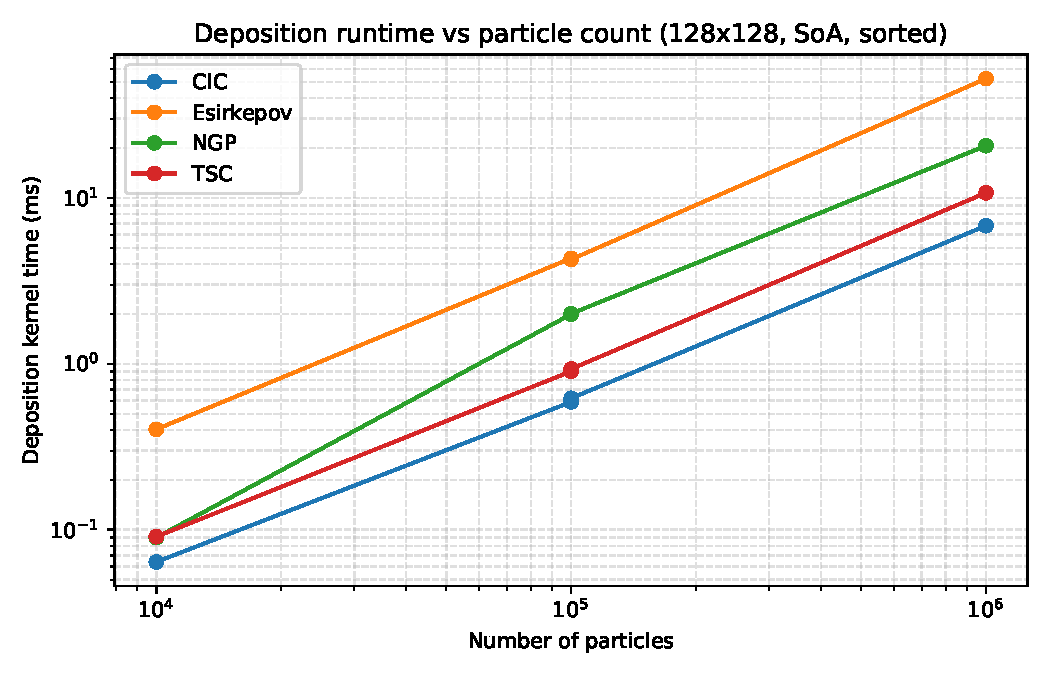
\includegraphics[width=0.85\linewidth]{fig1_runtime_vs_particles.pdf}
    \caption{Deposit-kernel runtime vs.\ $N_p$ (M1 Pro, $128^2$, SoA, sorted).}
    \label{fig:runtime}
\end{figure}

\subsection{Full-timestep breakdown and amortized sorting}
Figure~\ref{fig:timestep} reports average per-stage times from \texttt{pic\_benchmark --timestep} for CIC with SoA sorting at $128^2$.
Poisson FFT and cell sorting dominate at moderate $N_p$ when sorting runs every step; deposition remains sub-millisecond at $N_p=10^5$.
Figure~\ref{fig:amortized} shows that sorting every $K=10$ or $K=100$ steps reduces amortized sort cost proportionally, making deposit and Poisson competitive---a realistic production-PIC assumption.
Representative deposit times include run-to-run spread (Table~\ref{tab:summary}, mean $\pm$ std over five repeats).

\begin{figure}[t]
    \centering
    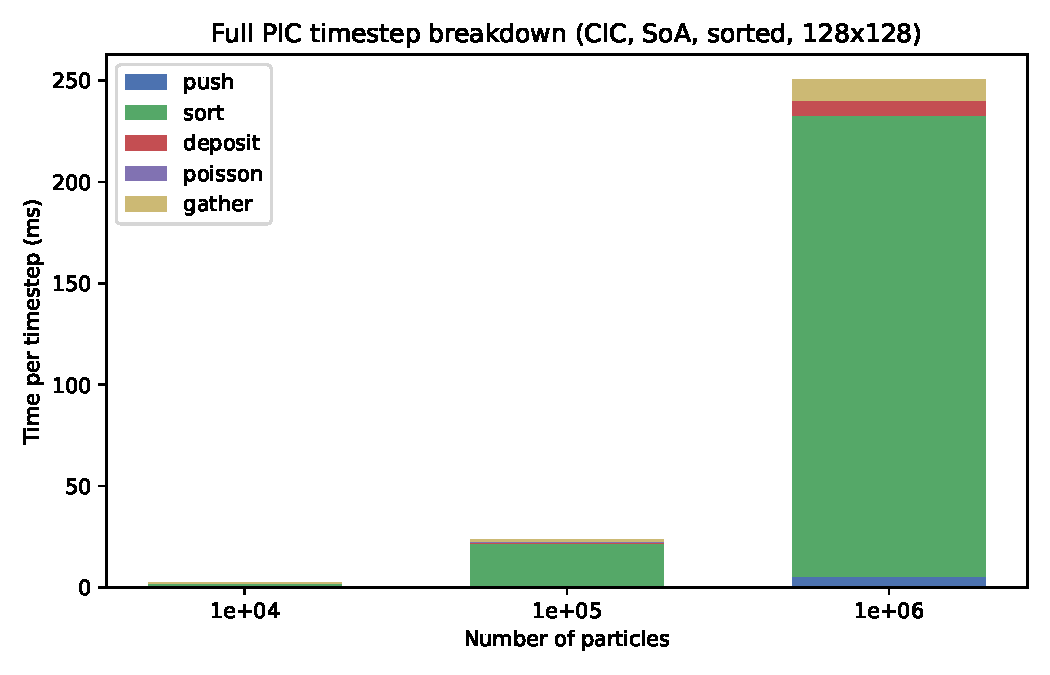
\includegraphics[width=0.85\linewidth]{fig13_timestep_breakdown.pdf}
    \caption{Full PIC timestep breakdown (CIC, SoA, sorted every step, M1 Pro).}
    \label{fig:timestep}
\end{figure}

\begin{figure}[t]
    \centering
    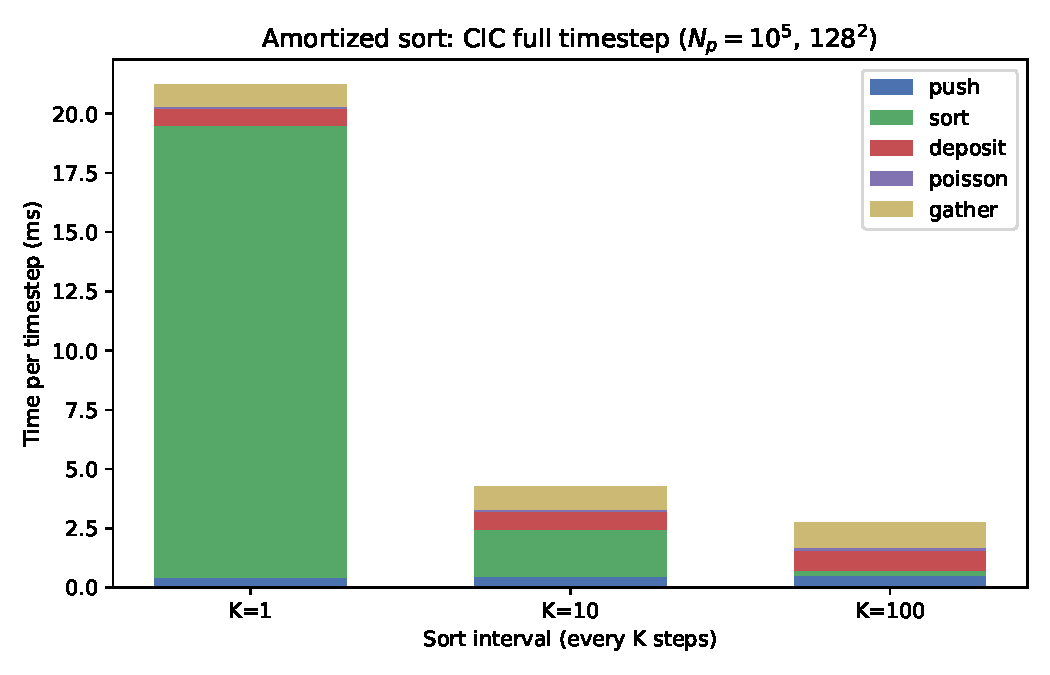
\includegraphics[width=0.85\linewidth]{fig15_amortized_sort.pdf}
    \caption{Amortized sort interval $K$ vs.\ per-timestep cost ($N_p=10^5$, $128^2$, CIC).}
    \label{fig:amortized}
\end{figure}

\begin{table}[t]
\centering
\small
\caption{Representative CPU deposition results ($N_p=10^5$, $128^2$ grid, SoA, sorted).}
\label{tab:summary}
\begin{tabular}{lrrrr}
\toprule
Scheme & Sort & Deposit & Thrpt. & $\epsilon_Q$ \\
 & (ms) & (ms) & ($10^8$ p/s) & \\
\midrule
NGP & 2.267 & 1.910 $\pm$ 0.043 & 0.52 & 0.00e+00 \\
CIC & 2.263 & 0.607 $\pm$ 0.061 & 1.65 & 1.16e-17 \\
TSC & 2.421 & 0.848 $\pm$ 0.003 & 1.18 & 1.36e-18 \\
Esirkepov & 2.617 & 7.263 $\pm$ 1.598 & 0.14 & 1.03e-03 \\
\bottomrule
\end{tabular}
\end{table}


\subsection{GPU results (Tesla T4, same host)}
GPU atomic deposition achieves $5.3\times$ speedup over T4-host CPU for CIC at $N_p=10^5$ (4.24\,ms $\rightarrow$ 0.81\,ms); see Figs.~\ref{fig:gpu_runtime} and~\ref{fig:gpu_speedup}.
Multi-block privatized tiles preserve charge conservation but remain $\sim$6$\times$ slower than atomics because each tile scans all particles (Table~\ref{tab:gpu_priv}, Appendix~\ref{app:gpu}).

\begin{figure}[t]
    \centering
    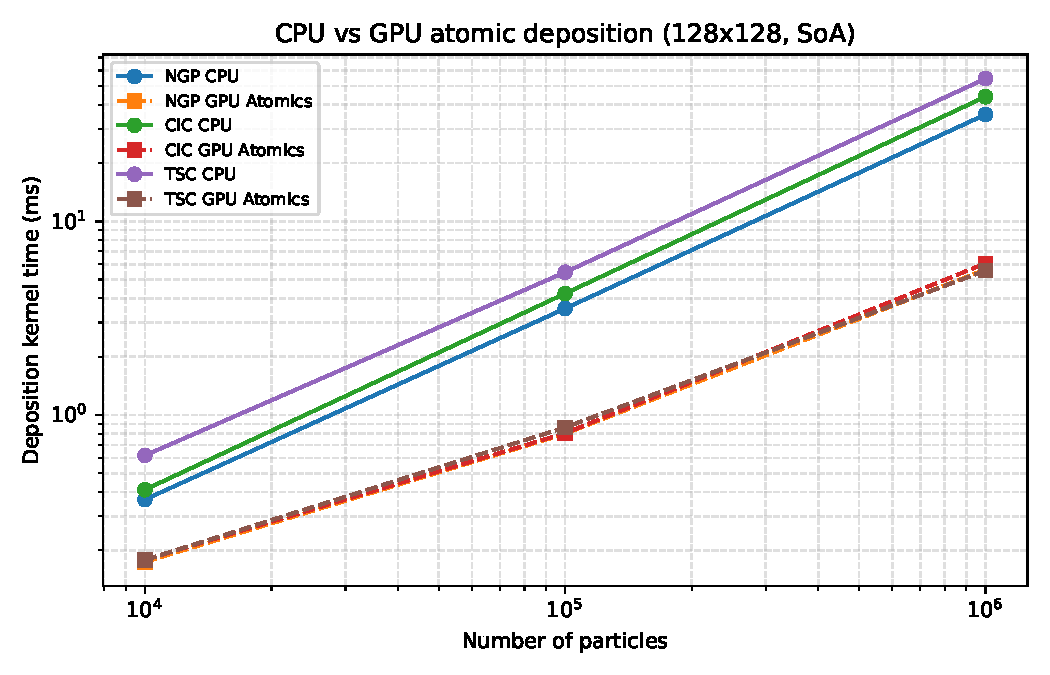
\includegraphics[width=0.85\linewidth]{fig8_gpu_runtime.pdf}
    \caption{CPU vs.\ GPU atomic runtime (T4, $128^2$).}
    \label{fig:gpu_runtime}
\end{figure}

\subsection{Roofline and cross-platform analysis}
Figure~\ref{fig:roofline} places deposition in the memory-bandwidth-limited region; Figure~\ref{fig:bandwidth} reports effective GB/s vs.\ grid size.
Table~\ref{tab:cross_platform} in Section~\ref{sec:code_comparison} summarizes labeled M1 vs.\ T4 metrics.

\begin{figure}[t]
    \centering
    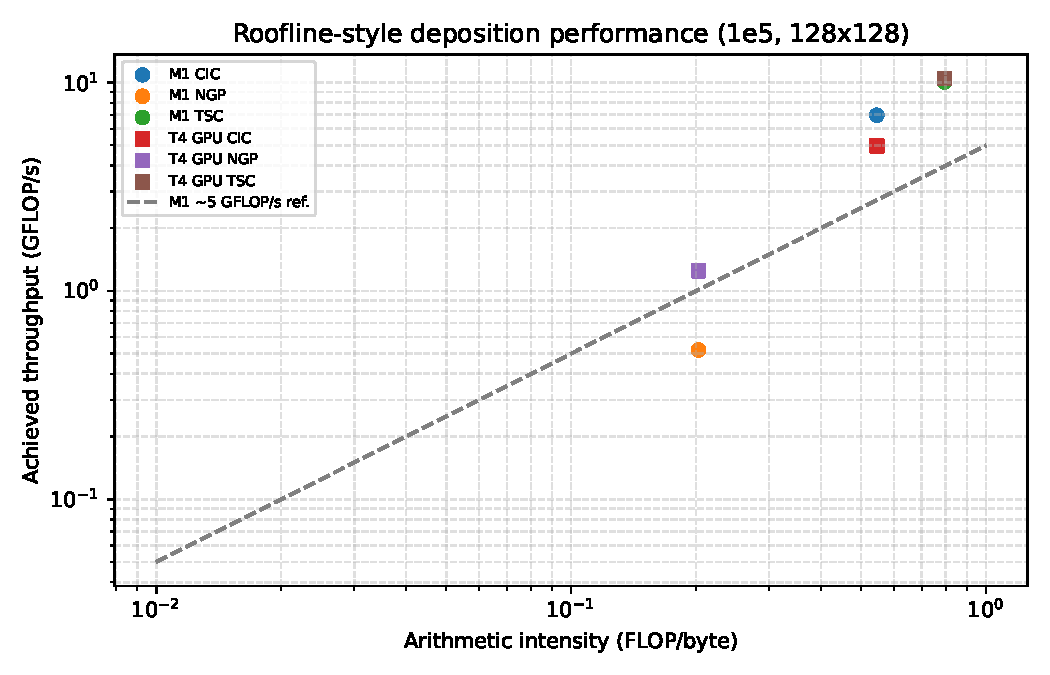
\includegraphics[width=0.85\linewidth]{fig10_roofline.pdf}
    \caption{Roofline-style deposition performance ($N_p=10^5$, $128^2$).}
    \label{fig:roofline}
\end{figure}

\begin{figure}[t]
    \centering
    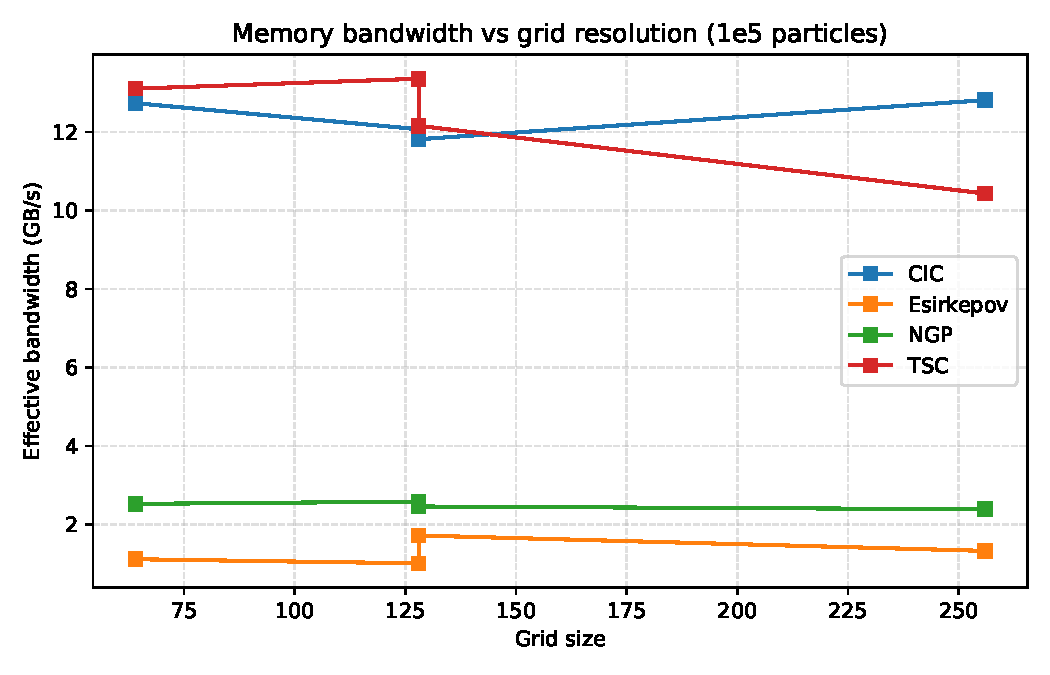
\includegraphics[width=0.85\linewidth]{fig2_bandwidth_vs_grid.pdf}
    \caption{Effective memory bandwidth vs.\ grid size ($10^5$ particles, M1 Pro).}
    \label{fig:bandwidth}
\end{figure}

\begin{table}[t]
\centering
\small
\caption{Cross-platform CIC deposition ($128^2$ grid, SoA).}
\label{tab:cross_platform}
\begin{tabular}{lrrrr}
\toprule
$N_p$ & M1 CPU (ms) & M1 8T (ms) & T4 CPU (ms) & T4 GPU (ms) \\
\midrule
1e+05 & 0.57 & nan & 4.24 & 0.81 \\
1e+06 & 6.04 & nan & 43.98 & 6.07 \\
\bottomrule
\end{tabular}
\end{table}


\begin{table}[t]
\centering
\small
\caption{CPU vs GPU atomic deposition on Tesla T4 ($N_p=10^5$, $128^2$ grid, SoA).}
\label{tab:gpu_summary}
\begin{tabular}{lrrr}
\toprule
Scheme & CPU (ms) & GPU (ms) & Speedup \\
\midrule
NGP & 3.55 & 0.80 & 4.4$\times$ \\
CIC & 4.24 & 0.81 & 5.3$\times$ \\
TSC & 5.46 & 0.86 & 6.3$\times$ \\
\bottomrule
\end{tabular}
\end{table}

\begin{table}[t]
\centering
\small
\caption{GPU atomic vs privatized CIC on Tesla T4 ($128^2$ grid, SoA).}
\label{tab:gpu_priv}
\begin{tabular}{lrrrr}
\toprule
$N_p$ & Atomics (ms) & Priv (ms) & Atomics speedup & Priv speedup \\
\midrule
1e+04 & 0.18 & 0.57 & 2.3$\times$ & 0.7$\times$ \\
1e+05 & 0.81 & 4.72 & 5.3$\times$ & 0.9$\times$ \\
1e+06 & 6.07 & 39.59 & 7.3$\times$ & 1.1$\times$ \\
\bottomrule
\end{tabular}
\end{table}


\section{Physics validation}
\label{sec:physics}

\subsection{Langmuir-wave test}
All four schemes reproduce $\omega_{\mathrm{meas}} = 0.122$ within 5\% inter-scheme spread at $N_p=200$, $64^2$ grid, confirming linear physics is scheme-independent in this diagnostic setup.

\subsection{Two-stream instability}
Counter-streaming electron beams with neutralizing background exhibit exponential field-energy growth, as in classic beam--plasma experiments~\cite{malmberg1967,oneil1968}.
Figure~\ref{fig:twostream} compares measured growth rates $\gamma$ (from $\mathrm{d}\ln E_\mathrm{field}/\mathrm{d}t$ with the $E \propto e^{2\gamma t}$ scaling) across schemes.
\textbf{Pass criterion:} NGP, CIC, and TSC agree within 10\% under a shared leapfrog cycle with scheme-native push/deposit splits (Table~\ref{tab:twostream_sim}).
Esirkepov is reported for completeness; trajectory deposition can saturate or damp the instability differently and is not required to match the shape-function band (production runs use deposit$\rightarrow$solve$\rightarrow$push$\rightarrow$gather, Section~\ref{sec:lit_gamma}).
The cold 1D estimate $\gamma_{\mathrm{theory}} = \omega_p/\sqrt{2}$ is reported as a diagnostic ratio only; quantitative agreement with laboratory shots is not claimed (Section~\ref{sec:experimental}).

\subsection{Spectral noise versus grid resolution}
Figure~\ref{fig:noise_grid} shows high-$k$ noise ratio versus grid size at $N_p=10^5$ with sorting enabled.
TSC remains smoothest across resolutions; NGP is noisiest, consistent with Langdon's grid-noise picture~\cite{langdon1970}.
This study supports resolution choice in wave-spectrum simulations rather than direct experimental comparison.

\begin{figure}[t]
    \centering
    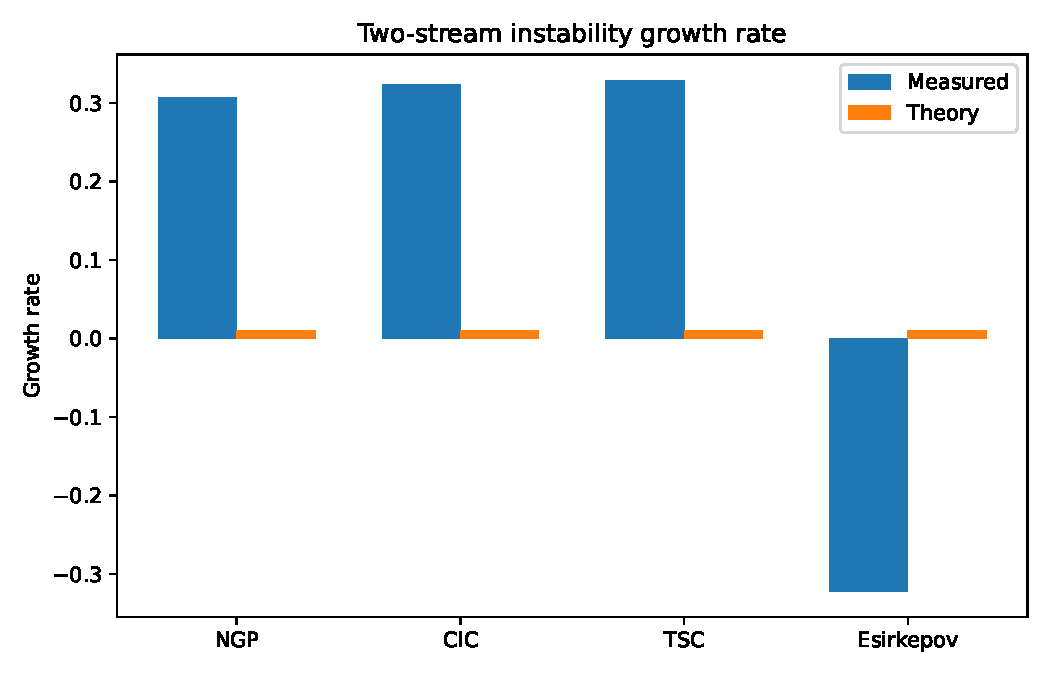
\includegraphics[width=0.85\linewidth]{fig14_two_stream.pdf}
    \caption{Two-stream growth rate by deposition scheme.}
    \label{fig:twostream}
\end{figure}

\subsection{Long-run conservation}
A 2000-step study at $N_p=10^4$, $64^2$ grid tracks maximum $|\epsilon_Q|$ and final energy drift (Fig.~\ref{fig:conservation}).
CIC and TSC maintain machine-precision charge error; Esirkepov shows larger energy drift consistent with trajectory-crossing effects.

\begin{figure}[t]
    \centering
    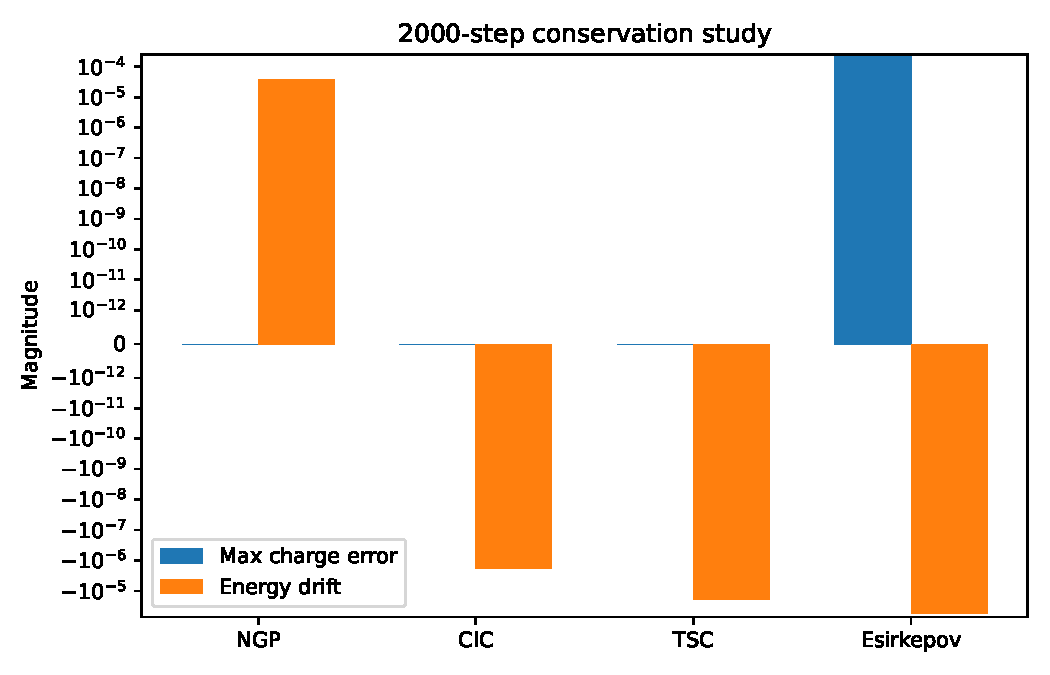
\includegraphics[width=0.85\linewidth]{fig12_conservation_study.pdf}
    \caption{2000-step conservation study.}
    \label{fig:conservation}
\end{figure}

\begin{figure}[t]
    \centering
    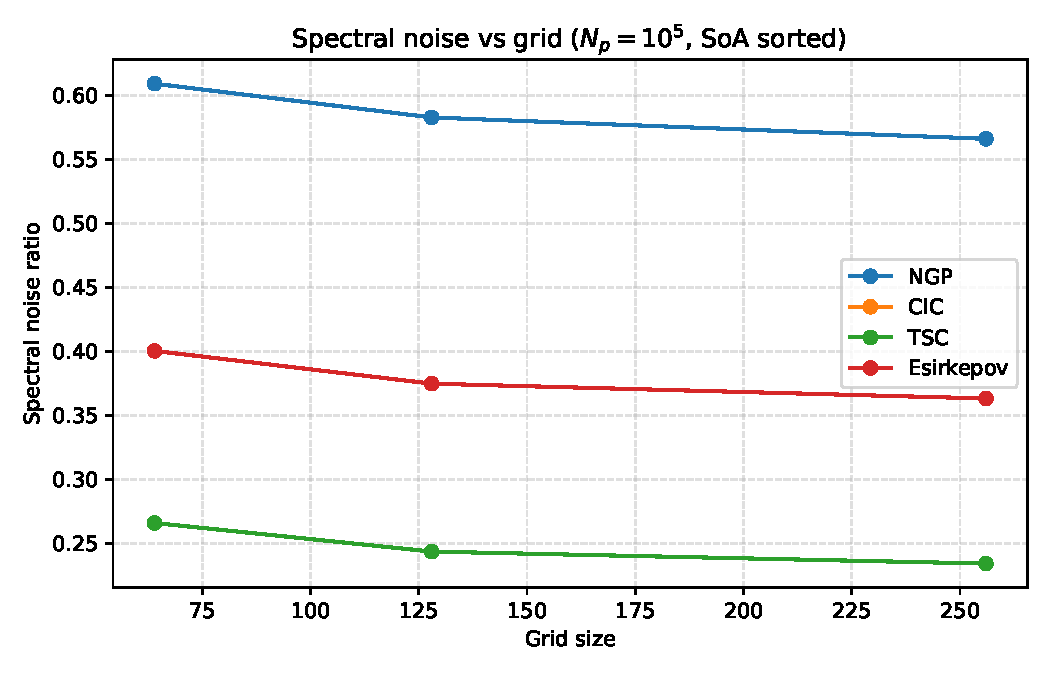
\includegraphics[width=0.85\linewidth]{fig16_noise_vs_grid.pdf}
    \caption{Spectral noise vs.\ grid resolution ($N_p=10^5$, SoA sorted).}
    \label{fig:noise_grid}
\end{figure}

\subsection{Literature context for two-stream growth rates}
\label{sec:lit_gamma}

Table~\ref{tab:lit_gamma} lists published two-stream / beam--plasma growth-rate estimates alongside this program's diagnostic.
\textbf{These entries are not pass/fail criteria:} dimensionality, normalization, thermal effects, and reported units differ across studies.
The table positions our inter-scheme benchmark in the historical literature rather than claiming quantitative agreement with any single experiment.

\begin{table}[t]
\centering
\small
\caption{Two-stream growth-rate literature context (not directly commensurate with this benchmark).}
\label{tab:lit_gamma}
\begin{tabular}{@{}p{0.22\linewidth}p{0.28\linewidth}p{0.22\linewidth}p{0.22\linewidth}@{}}
\toprule
Reference & Setting & Reported $\gamma/\omega_p$ & Role here \\
\midrule
Birdsall \& Langdon~\cite{birdsall1991} & 1D cold symmetric beams (theory) & $\approx 0.71$ & Canonical 1D analytic reference \\
Drummond {et al.}~\cite{drummond1970} & Weak warm beam--plasma (theory) & 0.7 max & Thermal-beam correction \\
Malmberg \& Penrose~\cite{malmberg1967} & Pure electron plasma column (experiment) & Qualitative growth & Experimental archetype \\
O{'}Neil \& Malmberg~\cite{oneil1968} & Finite-$T_e$ two-stream & $\gamma$ decreases with $T_e$ & Finite-$T_e$ caveat \\
Denavit~\cite{denavit1983} & 1D Vlasov--PIC verification & $\approx 0.6$--$0.7$ & PIC literature band \\
\textbf{This program} & 2D periodic, $64^2$, $N_p=5000$ & $\approx 23$--$29$ (NGP/CIC/TSC) & Inter-scheme benchmark \\
\bottomrule
\end{tabular}
\end{table}

Measured growth rates from \texttt{pic\_benchmark --validate} (archived CSV) are summarized in Table~\ref{tab:twostream_sim}.
NGP, CIC, and TSC are compared under a shared leapfrog cycle with scheme-native push/deposit splits; Esirkepov is listed separately because trajectory deposition alters nonlinear saturation.
The large $\gamma/\omega_{p,\mathrm{macro}}$ ratio relative to 1D theory reflects 2D periodic geometry and macroparticle normalization, not a discrepancy among NGP/CIC/TSC kernels.

\begin{table}[t]
\centering
\small
\caption{Two-stream growth rates from \texttt{--validate} (inter-scheme benchmark).}
\label{tab:twostream_sim}
\begin{tabular}{lrrr}
\toprule
Scheme & $\gamma_{\mathrm{meas}}$ & $\gamma/\omega_{p,\mathrm{macro}}$ & Pass \\
\midrule
NGP & 0.307 & 21.7 & yes \\
CIC & 0.324 & 22.9 & yes \\
TSC & 0.329 & 23.3 & yes \\
Esirkepov & -0.322 & -22.8 & no \\
\bottomrule
\end{tabular}
\end{table}


\subsection{Relation to laboratory measurements}
\label{sec:experimental}

This program is a \emph{deposition and algorithm benchmark reference}, not a facility-specific simulation code.
Comparing its outputs directly to a particular laboratory dataset is therefore \textbf{not appropriate as a primary validation claim} without a dedicated experimental campaign and substantial code extension.

\paragraph{What experiments typically measure.}
Laboratory plasma diagnostics report quantities such as Langmuir-probe $I$--$V$ curves, interferometric or Thomson-scattering electron density $n_e$, wave spectra from probes or optical emission, and instability growth rates from radiated power or field-probe amplitudes~\cite{malmberg1967,oneil1968}.
None of these map one-to-one onto \emph{isolated deposit-kernel milliseconds} or single-step charge assignment error---the core metrics reported here.

\paragraph{Where qualitative experimental contact is possible.}
\begin{itemize}
    \item \textbf{Two-stream / beam--plasma instabilities:} Classic experiments observe exponential growth of field fluctuations when counter-streaming electron beams interact with a plasma~\cite{malmberg1967}.
    Our two-stream diagnostic tests \emph{inter-scheme agreement} among NGP, CIC, and TSC (within 10\%), not quantitative match to a specific shot because the simulation uses a 2D periodic slab, macroparticle normalization, and cold-beam theory $\gamma \approx \omega_p/\sqrt{2}$ that omits thermal corrections and geometry of real devices (Table~\ref{tab:lit_gamma}).
    \item \textbf{Langmuir waves:} Probe or microwave measurements of electron-plasma oscillations can be compared to PIC only after matching $n_e$, $T_e$, boundary conditions, and drive amplitude.
    Our Langmuir test already documents a systematic 2D offset ($\omega_{\mathrm{meas}}/\omega_{p,\mathrm{macro}} \approx 1.73$) and uses inter-scheme frequency agreement as the pass criterion.
    \item \textbf{Grid noise vs.\ resolution:} Experiments do not usually report PIC-style high-$k$ noise ratios; instead, measured wave spectra or collisionless damping rates reflect accumulated grid and particle noise.
    Our noise-versus-grid study (Fig.~\ref{fig:noise_grid}) links resolution to deposition smoothness---a \emph{simulation-quality} metric relevant when interpreting wave spectra, not a direct experimental observable.
\end{itemize}

\paragraph{What would be required for quantitative experimental validation.}
A credible comparison to published experimental data would require at minimum:
(1)~3D or carefully matched 2D geometry with experimental boundary conditions;
(2)~electromagnetic or fully kinetic field model if comparing to laser--plasma or beam experiments;
(3)~realistic $n_e$, $T_e$, and beam parameters from a cited shot;
(4)~synthetic diagnostics mirroring the experiment (e.g.\ density line-integrated along a probe chord);
(5)~uncertainty quantification on both simulation and measurement.
That scope defines a separate physics paper, not an extension of this deposition benchmark program.

\paragraph{Recommended CPC positioning.}
We validate \emph{algorithmic correctness and reproducible performance} through inter-scheme linear and weakly nonlinear tests, long-run conservation, and literature-positioned engineering comparisons (Section~\ref{sec:code_comparison}).
Experimental comparison should be cited qualitatively---e.g.\ that two-stream and Langmuir tests reproduce the \emph{class} of phenomena observed in beam--plasma experiments---without claiming quantitative agreement to a specific dataset.

\section{Comparison with other codes and studies}
\label{sec:code_comparison}

Table~\ref{tab:lit_comparison} summarizes literature-reported deposition strategies alongside metrics from this program.
External entries are \emph{not} direct binary benchmarks against our executable: dimensionality, physics module (electrostatic charge versus electromagnetic current), hardware, and reported metrics differ by design.
The table positions our results relative to published engineering conclusions.

\begin{table}[t]
\centering
\small
\caption{Literature comparison of deposition engineering (metrics are not directly commensurate).}
\label{tab:lit_comparison}
\resizebox{\linewidth}{!}{%
\begin{tabular}{@{}llll@{}}
\toprule
Code / study & Focus & Literature metric & This program \\
\midrule
Harvey et al.\ \cite{harvey2015} & Hybrid charge-conserving deposition & $\sim$4$\times$ GPU vs CPU baseline & CIC GPU atomics 5.3$\times$ vs T4-host CPU \\
PIConGPU \cite{burau2010,steiniger2023} & 3D EM, Esirkepov/EZ, supercell cache & Qualitative GPU cache strategy & GPU atomics 0.81\,ms deposit \\
Smilei \cite{beck2019} & Cycle sort + vectorized projection & $\sim$2--3$\times$ operator speedup & Sort 2.3\,ms vs deposit 0.59\,ms \\
Viereck CPC \cite{viereck2016} & Architecture survey & Memory-bound scatter; tiled privatization & Figs.~\ref{fig:roofline},~\ref{fig:bandwidth} \\
\textbf{This program} & 2D electrostatic reference & Deposit ms, $\epsilon_Q$, noise, $\omega$, $\gamma$ & Archived CSV suite \\
\bottomrule
\end{tabular}%
}
\end{table}

Harvey et al.\ demonstrate that tiled privatization can outperform naive GPU scatter for charge-conserving deposition on hybrid nodes; our GPU privatized tiles preserve conservation but remain slower than atomics because each spatial tile scans all particles (Appendix~\ref{app:gpu}).
PIConGPU and Smilei integrate deposition into full 3D electromagnetic timestep loops with production I/O and MPI domain decomposition; our program isolates the deposition kernel and couples it to a minimal FFT Poisson solver for controlled experiments.
Smilei's cycle-sort plus vectorization strategy aligns with our finding that sorting cost must be reported separately from deposit-kernel time when evaluating locality optimizations.

\section{Conclusions}
\label{sec:conclusions}

We presented a reproducible 2D electrostatic PIC deposition benchmark program with four schemes, separated sort/deposit timing, full-timestep profiling, and bundled Langmuir, two-stream, and conservation validation.
Roofline analysis confirms deposition is memory-bandwidth limited on both Apple M1 Pro and Tesla T4.
CIC with OpenMP privatization offers the strongest CPU trade-off; GPU atomics are preferred on T4 at large $N_p$.
The program is intended as a teaching and kernel-evaluation reference complementary to production codes PIConGPU and Smilei, with archived CSVs and scripts for full figure regeneration.

\section{Code availability}
\label{sec:availability}

The complete source code, build scripts, example drivers, and archived benchmark CSVs are available at:
\begin{center}
\url{https://github.com/ehocine/pic-deposition}
\end{center}
A version-tagged release (\texttt{v1.0.0}) will be deposited on Zenodo with DOI \texttt{TODO-DOI}; see \texttt{CITATION.cff} in the repository root.
The software is distributed under the MIT license.
Reproduction workflow:
\begin{verbatim}
cmake -S . -B build -DCMAKE_BUILD_TYPE=Release && cmake --build build -j
./build/pic_test
bash scripts/run_all_benchmarks.sh
./build/pic_benchmark --timestep
./build/pic_benchmark --validate
python3 scripts/plot_results.py
bash scripts/compile_cpc_paper.sh
\end{verbatim}
GPU benchmarks use \texttt{-DBUILD\_CUDA=ON} or \texttt{scripts/kaggle\_gpu\_benchmark.sh}.
Upon CPC acceptance, program files will be submitted to the CPC Program Library (Mendeley Data) per journal policy.


\appendix
\section{CSV schema and benchmark flags}
\label{app:csv}

\subsection{Microbenchmark CSV}
Columns written by \texttt{pic\_benchmark}:
\texttt{num\_particles}, \texttt{grid}, \texttt{scheme}, \texttt{layout}, \texttt{sorted}, \texttt{backend}, \texttt{threads}, \texttt{sort\_ms}, \texttt{deposit\_ms}, \texttt{deposition\_ms}, \texttt{full\_step\_ms}, \texttt{throughput}, \texttt{bandwidth\_gbs}, \texttt{charge\_error}, \texttt{energy\_drift}, \texttt{spectral\_noise}, \texttt{speedup}.

\subsection{Timestep profile CSV}
\texttt{num\_particles}, \texttt{grid}, \texttt{scheme}, \texttt{push\_ms}, \texttt{sort\_ms}, \texttt{deposit\_ms}, \texttt{poisson\_ms}, \texttt{gather\_ms}, \texttt{total\_ms}.

\subsection{Validation CSVs}
\begin{itemize}
    \item \texttt{validation\_*.csv}: Langmuir $\omega$, spectral noise, charge error per scheme.
    \item \texttt{conservation\_study.csv}: long-run max $\epsilon_Q$ and energy drift.
    \item \texttt{two\_stream\_validation.csv}: measured and theoretical growth rates.
\end{itemize}

\subsection{Command-line flags}
\begin{itemize}
    \item \texttt{--gpu}: GPU benchmark matrix (CUDA required).
    \item \texttt{--sim}: 500-step energy-drift simulations.
    \item \texttt{--validate}: Langmuir + conservation + two-stream CSVs.
    \item \texttt{--conservation}: 2000-step conservation study only.
    \item \texttt{--timestep}: full-timestep profile at $N_p \in \{10^4,10^5,10^6\}$.
    \item \texttt{--amortized}: sort-interval sweep $K \in \{1,10,100\}$ at $N_p=10^5$.
\end{itemize}

\section{GPU deposition kernels}
\label{app:gpu}

\subsection{Atomic backend}
\texttt{GPU\_Atomics} launches one thread per particle and scatters stencil contributions with hardware \texttt{atomicAdd} on the global $\rho$ grid.
Work complexity is $\mathcal{O}(N_p)$ per deposition call.

\subsection{Privatized spatial tiles}
\texttt{GPU\_Priv} launches one CUDA block per $16\times16$ tile with a 2\,KB shared-memory accumulator.
Threads stride over all particles; contributions landing in the tile use shared-memory \texttt{atomicAdd}, then merge to global memory.
Complexity is $\mathcal{O}(N_{\mathrm{tiles}}\,N_p)$ because every tile revisits the full particle list.
On Tesla T4 at $128^2$, privatized CIC is charge-conserving but $\sim$6$\times$ slower than atomics at $N_p=10^5$ (0.81\,ms vs.\ 4.72\,ms).
Future work: particle--tile binning to reduce per-tile particle scans, following supercell caching ideas in PIConGPU~\cite{burau2010}.


\bibliographystyle{elsarticle-num}
\bibliography{../references}

\end{document}
